\documentclass[twoside,11pt]{article}

% Any additional packages needed should be included after jmlr2e.
% Note that jmlr2e.sty includes epsfig, amssymb, natbib and graphicx,
% and defines many common macros, such as 'proof' and 'example'.
%
% It also sets the bibliographystyle to plainnat; for more information on
% natbib citation styles, see the natbib documentation, a copy of which
% is archived at http://www.jmlr.org/format/natbib.pdf

\usepackage{jmlr2e}

\usepackage{listings}
% Definitions of handy macros can go here

\usepackage[dvipsnames]{xcolor}
\usepackage{wrapfig}

\lstset{
  language=Scala,
  basicstyle=\footnotesize\ttfamily,
  commentstyle=\color{gray},   
  frame=tb,
  numbers=left,
  numberstyle=\tiny,
  emph={%  
    val, def%
    },emphstyle={\bfseries\color{MidnightBlue}}%  
}

\newcommand{\todo}[1]{\textcolor{purple}{TODO: #1}}
\newcommand{\dataset}{{\cal D}}

% Heading arguments are {volume}{year}{pages}{date submitted}{date published}{paper id}{author-full-names}

\jmlrheading{1}{2000}{1-48}{4/00}{10/00}{meila00a}{Someone et al.}

% Short headings should be running head and authors last names

\ShortHeadings{Apache Mahout: Machine Learning on Distributed Dataflow Systems}{Meil\u{a} and Jordan}
\firstpageno{1}

\begin{document}

\title{Apache Mahout: Machine Learning on Distributed Dataflow Systems}

\author{\name Robin Anil \email robinanil@apache.org\\
  \name Gokhan Capan \email gcapan@apache.org\\
  \name Isabel Drost-Fromm \email isabel@apache.org\\
  \name Shannon Quinn \email squinn@apache.org\\
  \name Paritosh Ranjan \email pranjan@apache.org\\
  \name Sebastian Schelter \email ssc@apache.org\\
}

\editor{}

\maketitle

\begin{abstract}%   <- trailing '%' for backward compatibility of .sty file
Apache Mahout is a library for scalable machine learning (ML) on distributed dataflow systems, offering various implementations of classification, clustering, dimensionality reduction and recommendation algorithms. It originated in 2008 and targeted MapReduce, which was the predominant abstraction for scalable computing in industry at that time. It has since then migrated to a general framework for linear algebraic computations on dataflow backends such as Apache Spark, Apache Flink and H20. Mahout is maintained as a community-driven, top-level, open source project at the Apache Software Foundation. 
\end{abstract}

%\begin{keywords}
%  Bayesian Networks, Mixture Models, Chow-Liu Trees
%\end{keywords}

\section{Introduction}

\textit{Mahout} was started in 2008 as a subproject of the open source search engine \textit{Apache Lucence}~(\cite{Owen2012,Mccandless2010}), whose community encountered a growing need for applying ML techniques on large text corpora. In 2010, Mahout became a top-level Apache project. A critical component of modern large-scale machine learning (ML) is operating on, accessing, and analyzing datasets stored in distributed filesystems running on a cluster of machines. In such an environment, data analysis is often conducted using distributed dataflow engines, that allow for scalable, data-parallel execution of programs.

\section{Legacy: MapReduce-based Algorithms}
\todo{Clarify: Not many choices for ML in Hadoop ecosystem, quick introduction to MapReduce, (\cite{Chu2007}) showed that a large family of popular ML algorithms can be reformulated under the MapReduce paradigm}

Classification MR implementation of~\cite{Rennie2003}

Clustering MR implementation of canopy clustering~\cite{Mccallum2000}

Collaborative Filtering

SVD Lanczos + Stochastic SVD~\cite{Halko2012}

item-based collaborative filtering~(\cite{Sarwar2001}) \cite{Dunning1993,Schelter2012,Dunning2014},
ALS~\cite{Schelter2013} todo add original paper~\cite{Zhou2008}\\

\section{Mahout Samsara}

\todo{Intro, rewrite} Examples of such systems include Apache~Spark~(\cite{Zaharia2012}), Apache~Flink~(\cite{Alexandrov2014}) and H2o~(\cite{H2O}). Unfortunately, these systems are difficult to program, as their programming model is heavily influenced by the underlying data-parallel execution scheme. Usually, programs consist of a sequence of parallelizable second-order functions (such as \texttt{map}, \texttt{reduce} or \texttt{groupBy}) that dictate how the system should execute user-defined first-order functions on partitioned data~\cite{Zaharia2012}. Such programming models are non-intuitive for users without a background in distributed systems, and are in general hard to program without a detailed understanding of the underlying execution model. Furthermore, the available programming abstractions typically rely on partitioned, unordered sets; this is a mismatch for ML applications that mostly operate on linear algebra constructs (e.g.,~vectors and matrices). Therefore, implementing ML algorithms on dataflow systems is a tedious and difficult task. Mahout rebuilt itself on top of \emph{Samsara}~(\cite{Lyubimov2016}), a domain-specific language for declarative machine learning in cluster environments. Samsara allows its users to specify programs using a set of common matrix abstractions and linear algebraic operations, similar to R or MATLAB. Samsara then compiles, optimizes and executes these programs on distributed dataflow systems~(\cite{Schelter2016}). The aim of Samsara is to allow mathematicians and data scientists to leverage the scalability of distributed dataflow systems via common declarative abstractions, while drastically reducing the need for detailed knowledge of the programming model and execution scheme of the underlying systems. Samsara is part of the Apache Mahout library and supports backends like Apache Spark and Apache Flink. \todo{2 sentences for the optimization techniques}\\ 
%
\begin{wrapfigure}{r}{0.4\textwidth}
  \begin{center}
    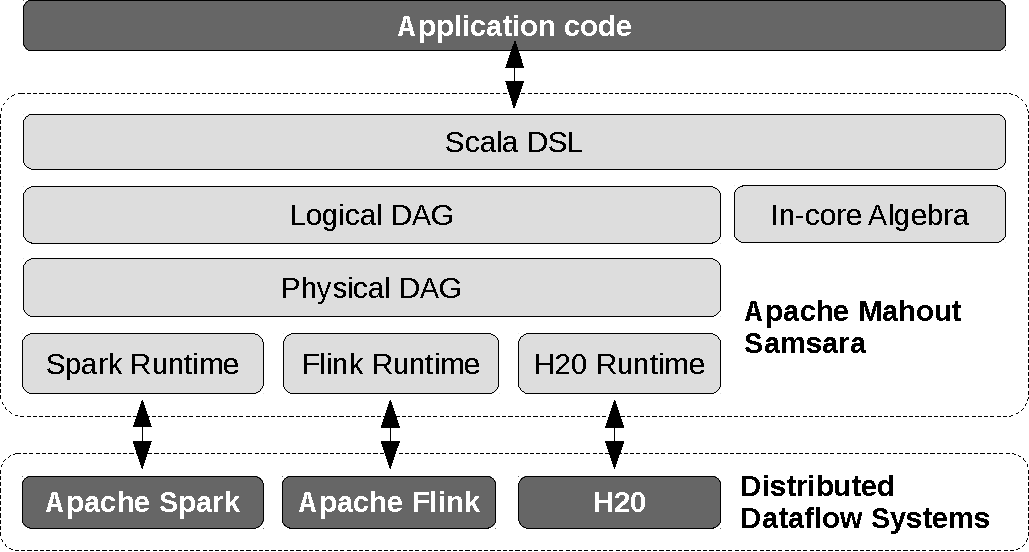
\includegraphics[scale=0.33]{figures/architecture-crop}
    \caption{Architecture.\label{fig:architecture}}
  \end{center}
\end{wrapfigure}
%
\noindent\textbf{Architecture and Execution}. Figure~\ref{fig:architecture} illustrates the architecture of Samsara. Applications are written using the Scala DSL. The in-memory operations are immediately executed, while operations on DRMs are deferred. The system records the actions to perform on these distributed matrices, and internally builds a directed acyclic graph (DAG) of logical operations from them, where vertices refer to matrices and edges correspond to transformations between them. Materialization barriers (e.g., persisting a result or collecting a matrix into local memory) implicitly trigger execution. Upon execution, the DAG of logical operators is optimized and transformed into a DAG of physical operators to execute. These physical operators are specific to one of the backends that Samsara supports (currently Apache~Spark and Apache~Flink), and run the distributed parts of the program using the respective backend. \todo{explain example in 3-4 sentences}

\begin{lstlisting}[numbers=left,numberstyle={\tiny},caption={Distributed Ridge Regression for tall \& skinny matrices using Samsara.},captionpos=b,label={lst:linearRegr}]
def dridge(data: DrmLike[Int], lambda: Double): Matrix {
  // slice out features, add column for bias term
  val drmX = data(::, 0 until data.ncol) cbind 1
  val drmY = data(::, data.ncol) // slice out target

  val drmXtX = drmX.t %*% drmX //distributed matrix
  val drmXtY = drmX.t %*% drmY // multiplications

  val XtX = drmXtX.collect // materialization of results
  val XtY = drmXty.collect // in driver memory

  XtX.diagv += lambda // add regularization
  solve(XtX, XtY) // compute parameters in-core on driver
}
\end{lstlisting}

\todo{Details on backends, e.g., Flink-backend~(\cite{Alexandrov2014}) has problems with control-flow}

\section{Availability and Requirements}

Mahout is run as a top-level project under the umbrella of the Apache Software Foundation, and developed in a community-driven, meritocratic fashion according to the \textit{Apache Way}\footnote{\url{https://www.apache.org/foundation/how-it-works.html}}. Mahout is available under an Apache License at \url{https://mahout.apache.org}. Mahout requires at least Java 7 and Scala 2.10 for Samsara. The legacy algorithms require Hadoop 2.4, while Samsara compiles to to Flink 1.1, Spark 1.6/2.x and H20 0.1.25.

\section{Outlook}

linear + relational algebra, df systems one extreme, dl systems other, middleground must be found

\section{Acknowledgements}
\todo{list anyone here who chose not to be a co-author} Mahout is the product of the efforts of numerous people. We would like to thank all the project's committers who did not co-author this paper: Abdelhakim Deneche, Anand Avati, Andrew Musselman, Benson Margulies, Dan Filimon, David Hall, Dawid Weiss, Dmitriy Lyubimov, Drew Farris, Ellen Friedman, Erik Hatcher, Frank Scholten, Grant Ingersoll, Jake Mannix, Jeff Eastman, Karl Wettin, Niranjan Balasubramanian, Otis Gospodnetic, Ozgur Yilmazel, Pat Ferrel,  Sean Owen, Stevo Slavić, Suneel Marthi, Ted Dunning, Tom Pierce, Trevor Grant. Of course we extend our thanks tos all users and contributors as well.

\vskip 0.2in
\bibliography{mahout}

\end{document}
 